\textbf{Anchoring on the table fails from overhead.} All four relative models
have a median volume error of 92.7--99.4\,\% under the deployable anchor
protocol (Table~\ref{tab:n5k}), even though their predicted table is flat to
0.6--0.7\,mm RMS: the affine fit reproduces the table and collapses the food
relief. The anchor fit is badly conditioned on most dishes
(Fig.~\ref{fig:cond}), as expected when the only reference is a plane almost
perpendicular to the optical axis. This is the quantitative reason the rig
views the plate at $45^\circ$ and uses the marker mat and multiple views.

\textbf{Metric models are not metric at plate distance.} Used as-is, the three
DA-V2 metric indoor models have AbsRel 1.33--2.03 and a median volume error of
759--801\,\%: 36\,cm is far outside the room-scale depths they were trained on.
After anchoring, the small model reaches 73.5\,\% [67.3, 80.3], the lowest
anchor error of the seven models, but its predicted table is not flat
(11\,mm RMS against 0.6\,mm for the relative models) and only 12\,\% of dishes
fall within 20\,\%. Under the oracle fit all three metric models
(75--100\,\%) are worse than every relative Depth Anything model. Model size
does not order them: B is the worst of the three under every protocol.

\textbf{Depth metrics do not predict volume.} After alignment AbsRel is
0.015--0.125 for every model, yet volume errors span 13--100\,\%. Food relief
(1--3\,cm) is a small fraction of the 36\,cm camera distance, so a model can
score well on depth and still lose most of the volume. We therefore rank
models on volume, not on AbsRel.

\textbf{Oracle upper bound.} With an oracle fit DA-V2-B is best of all seven models: 32.1\,\%
[28.5, 35.7] median volume error with its own support plane and 13.0\,\% with
the sensor's plane. Paired Wilcoxon tests with Holm correction separate it from
DA-V2-S ($p=8.6\times10^{-10}$), DA-V1-S ($p=7.8\times10^{-18}$) and
MiDaS-DPT-Hybrid ($p=2.2\times10^{-55}$). Within Depth Anything V2, the larger
encoder helps (B over S), but the gain is small next to the gap between
protocols. The gap between the two plane choices shows that
fitting the support plane in predicted depth causes more than half of the
error; in the rig the marker mat provides this plane independently of the
network.

\textbf{Coverage and failures.} 498 of the 503 usable dishes were evaluated
for every model. The remaining five have no visible table
(degenerate plane fit) and are counted as failures, not dropped. Latency is
1.4--3.8\,s per image on 8-vCPU cloud VMs (VM evidence): the relative models
ran on a machine shared with other jobs, so their times are upper bounds, and
the metric models ran alone on an identical second VM. ZoeDepth, DA-V2-L
(relative) and Depth Pro are implemented in the same benchmark but had not
finished at the time of writing.
\begin{figure}[t]
\centering
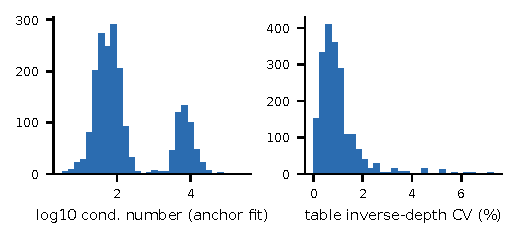
\includegraphics[width=\columnwidth]{figs/n5k_anchor_conditioning.pdf}
\caption{Anchor-fit conditioning on Nutrition5k (relative models): condition
number of the affine fit (left) and coefficient of variation of table inverse
depth (right). A low CV means the table alone cannot separate scale from shift.}
\label{fig:cond}
\end{figure}
